\documentclass[a4paper, 11pt]{article}
\usepackage{comment} % enables the use of multi-line comments (\ifx \fi) 
\usepackage{lipsum} %This package just generates Lorem Ipsum filler text. 
\usepackage{fullpage} % changes the margin
\usepackage{amsmath}
\usepackage{epstopdf}
\usepackage{graphicx}


\title{Sparse Regression}
\date{}
\begin{document}
\author{}
\maketitle
%Header-Make sure you update this information!!!!
\noindent
\large\textbf{Team 4} \hfill \textbf{Natali Alfonso, Simon Kern, Vangelis Kostas} \\
\normalsize Machine Learning (NWI-NM048C)  \\
Prof. B. Kappen\hfill Due date: 31/01/2017 \\


\subsection*{Introduction}
A regression is formulated as a mapping from a matrix A to outcomes b, where A consist of rows of observations. Now it is the task to find multiplication coefficients for each column (feature) in A to find or approximate the mapping: $argmin_x(b=Ax)$. With the found coefficients (or weights) we can now create output values for unseen data.\\
In the case of a square matrix we can usually find an analytical solution for the problem, but if we have more features than patterns our linear equation system is under-determined and hence we easily overfit, leaving it hard to interpret the weights. Different regularization terms have been proposed to filter out the features that are less important or correlated. One such approach is Lasso regression which implements an L1 regularization. Lasso drives some of the coefficients to zero, leaving only more important coefficients behind. The sparsity of the solution set makes it easier to interpret the results. The L2 regularization is called Ridge regression, where less important coefficients are driven towards 0, but never reach it.

\subsection*{Derivation of the Gauss-Seidel update rule}
The Gauss-Seidel update rule is given by 
  \begin{equation}
  x^{'}_i=\frac{1}{A{ii}}(b_i-\sum_{j>i}A_{ij}x_j-\sum_{j<i}A_{ij}x^{'}_j)
  \end{equation}
\\\\
We start with a normal regression formula $b = Ax$. Where $b$ is our target, $A$ is the design matrix consisting of columns of features and rows of data points and $x$ our regression coefficients.\\
Now lets decompose $A$ into it's upper and lower part \begin{equation}
L = A_{ij}, j\leq i \quad \textrm{and} \quad      U=A_{ij}j>i
\end{equation}.\\
Our original equation is now
\begin{equation}
\begin{split}
b & = (L+D)x \\
b & = Lx'+Dx\\
\end{split}
\end{equation}
With our initial definition of $L$ and $D$ we can write for each row $i$ in $A$ (for each row in the equation system) \\
\begin{equation}
\begin{split}
b_i & = \sum_{j>i}A_{ij}x_j - \sum_{j\leq i}A_{ij}x_j'\\
b_i & = \sum_{j>i}A_{ij}x_j - (\sum_{j<i}A_{ij}x_j' + A_{ii}x_i')\\
A_{ii}x_i' & = b_i -\sum_{j>i}A_{ij}x_j - \sum_{j<i}A_{ij}x_j'\\
 x^{'}_i &=\frac{1}{A{ii}}(b_i-\sum_{j>i}A_{ij}x_j-\sum_{j<i}A_{ij}x^{'}_j)
\end{split}
\end{equation}
Which is the Gauss-Seidel update rule.



\subsection*{Write your own Lasso method}
For the LASSO we have the following function that we want to minimize:
\begin{equation}
 E(\beta) = \frac{1}{2}||y-A\beta||^2+\lambda||x||_1
\end{equation}
A usual approach to this problem is using the Jacobi-Method in which we go through the equation system and solve each equation for exactly one unknown, keeping the others fixed.


\begin{equation}
\begin{split}
x_i & = \frac{1}{A{ii}}(b_i-\sum_{j\neq i}A_{ij}x_j)
\end{split}
\end{equation}
If our matrix $A$ is not not square, that means for instance we have less patterns than features, the algorithm would not have enough rows to perform this update.\\
We implemented a variation of that method that performs the update per $x_i$ not for one, but for all patterns and takes the average of the updates for a new value of $x_i$\\

\begin{equation}
\begin{split}
\hat{x_i} & = \frac{1}{p} \sum_p \frac{1}{A_{pi}}(b_p-\sum_{j,j\neq i}A_{pj}x_j)
\end{split}
\end{equation}
To accomodate for a L1 regularization (Lasso) we used the following update rule as given by the slides:
\begin{equation}
x_i = sign(\hat{x_i})(|\hat{x_i}|-\lambda)_+
\end{equation}
And used an regular Mean Square Error (MSE) as a performance measure.

\subsection*{Test of the Lasso algorithm}
We are given two datasets, train and validation. We initialize our betas to $\beta\sim U(\pm 1)$ to ensure a warm start. As suggested in the literature we use an early stopping criteria of $\frac{||\beta_t - \beta_{t-1}||}{||\beta_t||}<0.01$, as a measurement of stagnation of change in $\beta$, or run for 100 iterations.
We used a 5-fold cross validation on the train set to find out the best value for $\lambda$. Additionally we calculated $\beta$-coefficients on the entire train set and tested them on the validation set for log spaced $\lambda$ values from 0 to 1.
Our best $\lambda$ value found via cross-validation was $0.14678$. This appears to be slightly higher than the optimal lambda found on the validation set. Results can be seen in Figure \ref{img:lambda}


\begin{figure}[htbp]
\hspace{-3.5cm}
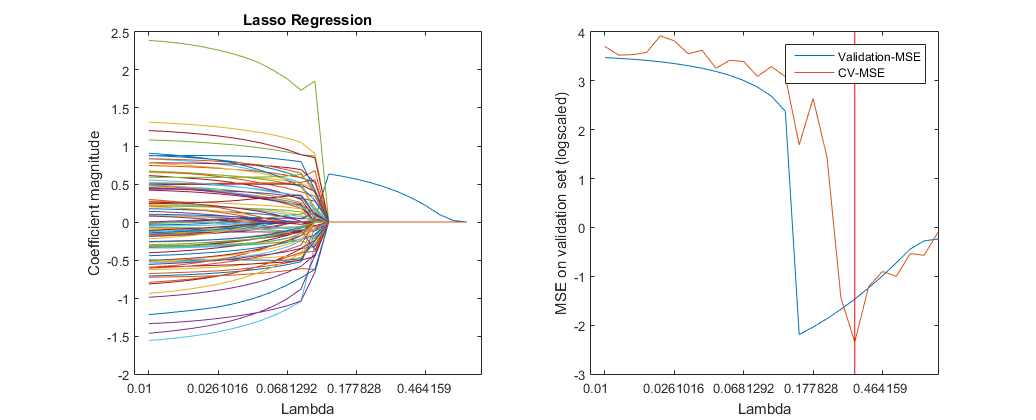
\includegraphics[scale=0.8]{lasso.png}
\caption{Coefficients and MSE for different lambda-values for Lasso}
\label{img:lambda}
\end{figure}

\subsection*{Ridge Regression}
To compare our results to Ridge regression, we did a 5-fold cross validation to find the optimal value $k$ for Ridge using the Matlab built-in Ridge regression function. Results can be seen in Figure \ref{img:k}. The coefficients approach zero in a smooth manner, but never quite reach it. Our best value for $k$ turned out to be $46.6$, with the lowest MSE on the cross validation. 
\begin{figure}[htbp]
\hspace{-3.5cm}
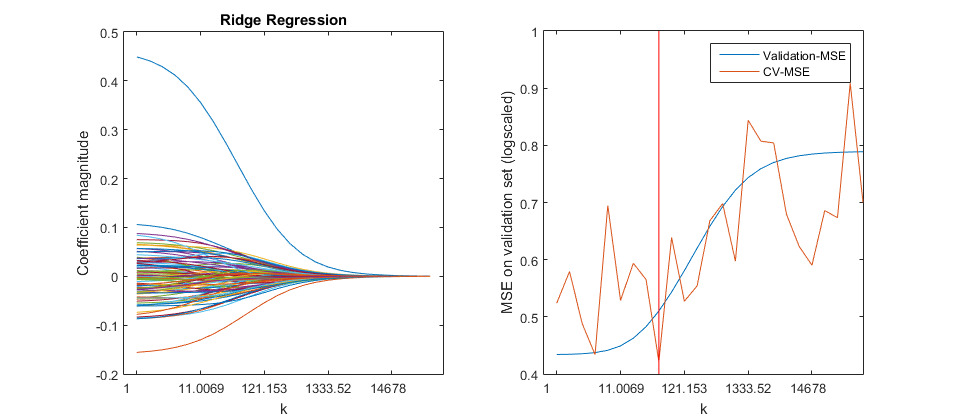
\includegraphics[scale=0.8]{ridge.png}
\caption{Coefficients for the optimal lambda}
\label{img:k}
\end{figure}

\subsection*{Comparing Ridge to Lasso}

We observe that the final $\beta$-values for Lasso are much sparser than for Ridge. Most of them are in fact 0. This behaviour is exactly as expected. On the other side we see that Ridge regression weights are all relatively small and distributed over all $\beta$. Ridge does not force weights to go to zero. See Figure \ref{img:weights}
\begin{figure}[htbp]
\hspace{-3.5cm}
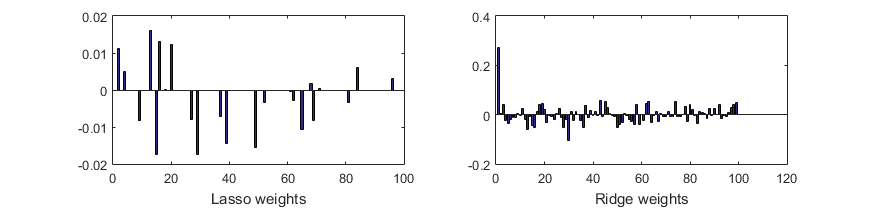
\includegraphics[scale=0.9]{weights.png}
\caption{Coefficients and MSE for different lambda-values for Lasso}
\label{img:weights}
\end{figure}

\subsection*{Correlated inputs}
When our design matrix $A$ has strongly correlated features Lasso might give results which are not following the ordering of the feature importance in the data. We used a toy case (see slides p.222) to observe this behaviour.\\
We run the same procedure as above (5-fold cross validation,..) using data created with the provided Matlab script. Two examples are given, 1a with weights [2,3,0] and 1b with [-2,3,0]. Results of the trace-plot can be seen at Figure \ref{img:corr} and for 1b at Figure \ref{img:corr1b}.\\We find best $\beta$ values of [2.15; 3.04; -0.1] for 1a, which do not correspond to the real correlations [1.83; 2.74 ;3.02] ($b=\frac{1}{p}xy$). For 1b we find [-2.20;2.80;0.20] for our $\beta$. These are surprisingly close to the real correlations [-2.12; 2.98; 0.55]. In 1a we assume the wrong order of $\beta$ values is because of the matching sign of $\beta_1, \beta_2$. As the sign of the values is opposite in case 1b, we observe a correct ordering of the weights. These results reflect considerations of Zhao and Yu (2004).

\begin{figure}[htbp]
\hspace{-3.5cm}
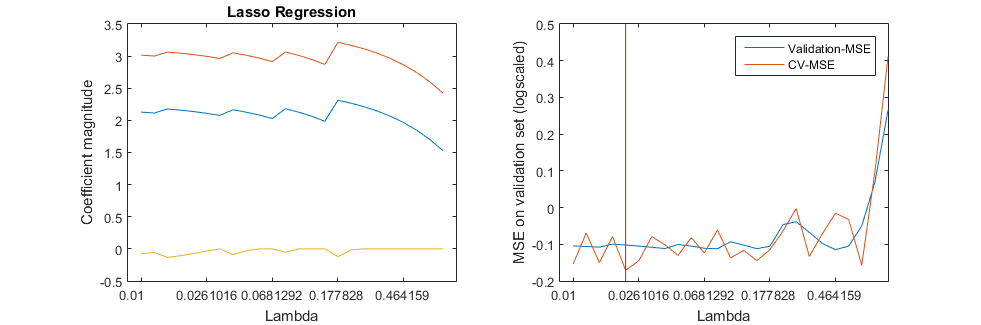
\includegraphics[scale=0.8]{correlated.png}
\caption{Coefficients and MSE for correlated case using Lasso for weights [-2,3,0]}
\label{img:corr}
\end{figure}

\begin{figure}[htbp]
\hspace{-3.5cm}
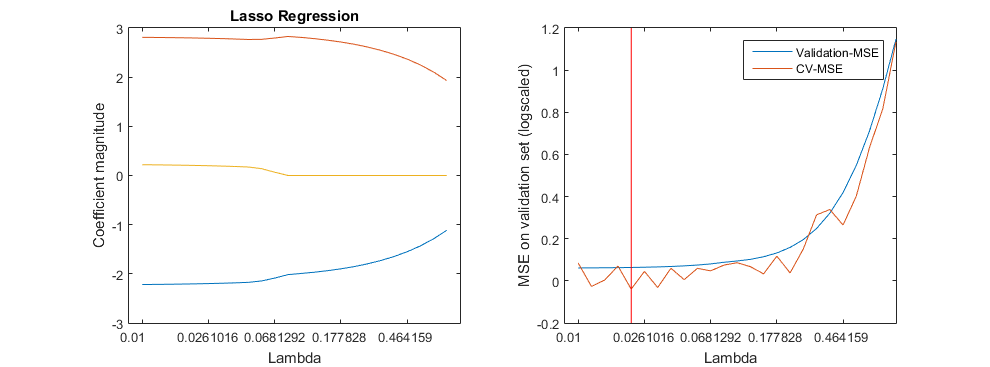
\includegraphics[scale=0.8]{correlated1b.png}
\caption{Coefficients and MSE for correlated case using Lasso for weights [2,3,0]}
\label{img:corr1b}
\end{figure}

\subsection*{Discussion}
We compared two different regularization techniques for performing a regression: Ridge and Lasso. As expected, Lasso can select important features by setting unimportant feature-coefficients to zero, leading to a sparse solution. This is particularly useful for under-determined systems. Ridge regression can also constrain our weights in magnitude, but never sets them to zero, leaving the result hard to interpret. Lasso has problems if the input data is highly correlated, were ordering of coefficients can be wrong if there exists a sign inconsistency. Even though we can confirm these findings, we are surprised, that the found coefficients are quite close to the initial weights. Problems with correlated data can be circumvented by using an Elastic net, which is a mixture between the $L1$ and the $L2$ norm


\end{document}
